\usepackage{amsmath}
\usepackage{amssymb}
\usepackage{amsthm}
\usepackage{changepage}
\usepackage{graphicx}
\usepackage{hyperref}
\usepackage{tikz}
%\usepackage{newtxtext,newtxmath} % Times-like font
\usepackage{pgfplots}
\pgfplotsset{compat=1.18} % or 1.17, etc.
\usepackage{booktabs} % for nicer table lines
\usepackage{titling}

\theoremstyle{plain}
\newtheorem{theorem}{Theorem}[section]
\newtheorem{lemma}[theorem]{Lemma}
\newtheorem{corollary}[theorem]{Corollary}
\theoremstyle{definition}
\newtheorem{definition}[theorem]{Definition}
\newtheorem{example}[theorem]{Example}
\newtheorem{properties}[theorem]{Properties}

\newcommand{\nextp}{\par\bigskip}

\setlength{\parindent}{0pt}


% Header + Footer
\fancyhf{}
\rhead{AP Statistics Notes}
\lhead{Exploring One-Variable Data}
\cfoot{\thepage}

% Title
\title{
  AP Statistics Notes\\[1ex]
  \large Unit 1: Exploring One-Variable Data
}
\author{}
\date{}

\begin{document}

\maketitle


\section*{Overview}
You'll be introduced to how statisticians approach variation and practice representing data, describing distributions of data, and drawing conclusions based on a theoretical distribution.
\bigskip


\section*{1.1 What Can We Learn from Data?}
\textbf{Statistics} is the science of collecting, organizing, analyzing, and interpreting data to make decisions or answer questions. \\
\begin{tcolorbox}[title=Key Terms, colback=blue!5!white, colframe=blue!75!black, breakable]
\begin{itemize}
    \item \textbf{Individual:} A single unit from which data is collected (e.g., a person, object). 
    \item \textbf{Variable:} A characteristic or measurement that varies from one individual to another.
    \item \textbf{Population:} The entire set of individuals we want to study.
    \item \textbf{Sample:} A subset of the population from which we actually collect data.
\end{itemize}
\end{tcolorbox} 
In statistics, we collect sample data on certain variables using measurements on individuals. \\
\par\medskip
\textbf{Example:} A researcher surveys a random sample of 250 college students to examine their study habits. In this study, the population is all college students and the sample is the subset of 250 who took the survey. The variable here would be ``hours studied per week" or some similar quantity of interest.
\bigskip


\section*{1.2 Variables and Types of Data}
\begin{tcolorbox}[title=Key Terms, colback=blue!5!white, colframe=blue!75!black, breakable]
\begin{itemize}
    \item \textbf{Categorical/Qualitative Variable:} A variable that can take on one of a limited, usually fixed number of possible ``classes" or group labels.
    \item \textbf{Numerical/Quantitative Variable:} A variable that takes on number values, from a measured or counted quantity, and can be analyzed using arithmetic. 
\end{itemize}
\end{tcolorbox}
Numerical variables can be further split into either discrete or continuous variables.
\begin{tcolorbox}[title=Key Terms, colback=blue!5!white, colframe=blue!75!black, breakable]
\begin{itemize}
  \item \textbf{Discrete Variable:} Have a countable set of possible number values
  \item \textbf{Continuous Variable:} Takes on an infinite range of possible values
\end{itemize}
\end{tcolorbox}
\par\medskip
\textbf{Example:}
\begin{itemize}
  \item Ethnicity: Categorical
  \item Income: Quantitative (continuous)
  \item High school class: Categorical
  \item Age in years: Quantitative (discrete) 
\end{itemize}
\bigskip


\section*{1.3--1.4 Representing Categorical Data with Tables and Graphs}
Tables can be used to summarize data and get a quick overview of our data. 
\begin{tcolorbox}[title=Key Terms, colback=blue!5!white, colframe=blue!75!black, breakable]
\begin{itemize}
    \item The \textbf{frequency} of a value is just how many times that value occurs among our data.
    \item The \textbf{relative frequency} ($rf$) of a value is the ratio of its frequency to the total number of observations, $n$.
    \item The \textbf{cumulative frequency} ($cf$) of a value uses the number of observations less than or equal to that value. (This is useful when the possible values are \textit{ordered} in some way.)
    \item We could similarly calculate the \textbf{relative cumulative frequency}.
    \item A \textbf{frequency table} gives the number of cases falling into each category. A \textbf{relative frequency table} includes the proportion of cases falling into each category.
\end{itemize}
\end{tcolorbox}
\par\medskip
\textbf{Frequency Table}
\begin{center}
\begin{tabular}{lcc}
\toprule
Pet & Frequency & Relative Frequency \\
\midrule
Dog & 20 & 0.40 \\
Cat & 15 & 0.30 \\
Fish & 10 & 0.20 \\
Other & 5 & 0.10 \\
\bottomrule
\end{tabular}
\end{center}
\par\medskip
Of course, to get a better view of the data, we will want to use charts and graphs too. Here are some examples of graphs that are widely used for \textbf{data visualization}. \\
\par\medskip
\textbf{Bar Chart}
\begin{center}
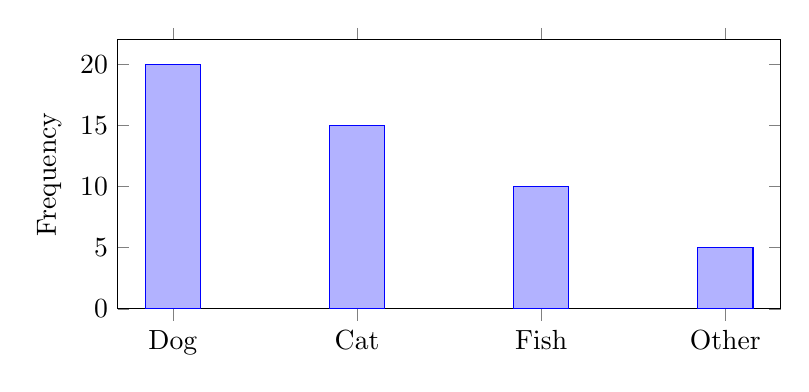
\begin{tikzpicture}
\begin{axis}[
    ybar,
    ymin=0,
    ylabel={Frequency},
    symbolic x coords={Dog, Cat, Fish, Other},
    xtick=data,
    bar width=20pt,
    width=10cm,
    height=5cm
]
\addplot coordinates {(Dog,20) (Cat,15) (Fish,10) (Other,5)};
\end{axis}
\end{tikzpicture}
\end{center}
\textbf{Pie Chart}
\begin{center}
\begin{tikzpicture}
\pie[radius=2]{62/In-state, 23/Out-of-state, 15/International}
%\caption{Pie chart displaying types of student residency at a college}
\end{tikzpicture}
\end{center}
\bigskip


\section*{1.5 Representing Quantitative Data  with Tables and Graphs}
\textbf{Dotplot}
\begin{center}
\begin{tikzpicture}
\begin{axis}[
    width=12cm,
    height=4.5cm,
    xlabel={Shoe Size},
    axis lines=left,
    xtick={7,8,9,10,11,12,13,14},
    xmin=6.5, xmax=14.5,
    ytick=\empty,
    ymin=0, ymax=4,
    enlargelimits=false,
    clip=false,
    ticklabel style={font=\small}
]

% Example data: shoe sizes with stacked dots
\addplot+[only marks, mark=*, mark size=2pt] 
coordinates {
    (7,1) 
    (8,1) (8,2) 
    (9,1) (9,2) (9,3) 
    (10,1) (10,2)
    (11,1)
    (12,1) (12,2)
    (13,1)
    (14,1)
};

\end{axis}
\end{tikzpicture}
\end{center}

\textbf{Histogram}
\begin{center}
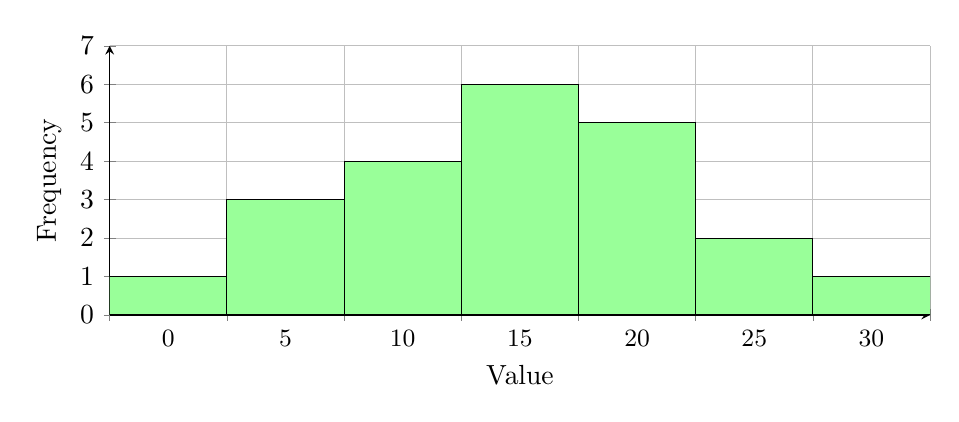
\begin{tikzpicture}
\begin{axis}[
    ybar interval,
    ymin=0,
    ymax=7,
    xmin=0,
    xmax=35,
    axis x line=bottom,
    axis y line=left,
    xlabel={Value},
    ylabel={Frequency},
    xtick={0,5,10,15,20,25,30,35},
    ytick={0,1,2,3,4,5,6,7},
    width=12cm,
    height=5cm,
    bar width=0.8,
    xticklabel style={font=\small},
    ymajorgrids=true
]
% Bin edges and frequencies: (left edge, frequency)
\addplot+[
    draw=black,
    fill=green!40
] coordinates {
    (0,1)
    (5,3)
    (10,4)
    (15,6)
    (20,5)
    (25,2)
    (30,1)
    (35,0)
};
\end{axis}
\end{tikzpicture}
\end{center}

\textbf{Boxplot}
\begin{center}
\begin{tikzpicture}
\begin{axis}[
    boxplot/draw direction=x,
    height=3.5cm,
    width=10cm,
    ytick={1},
    yticklabels={Test Scores},
    xlabel={Value},
    xmin=0, xmax=100,
    xtick={0,20,40,60,80,100},
    xticklabel style={font=\small},
    grid=major
]
\addplot+[
    boxplot prepared={
        lower whisker=25,
        lower quartile=35,
        median=50,
        upper quartile=70,
        upper whisker=85
    },
    draw=black,
    fill=orange!30
] coordinates {};
\end{axis}
\end{tikzpicture}
\end{center}

\textbf{Stemplot}
\begin{center}
\begin{tabular}{ll}
\textbf{Stem} & \textbf{Leaf} \\
\hline
2 & 3 \\
3 & 1 4 8 \\
4 & 0 2 5 \\
5 & 0 7 \\
6 & 1 \\
\end{tabular}
\end{center}
\bigskip


\section*{1.6 Describing the Distribution of Quantitative Data}
When it comes to quantitative variables, we will want to discuss certain important characteristics of distributions.
\begin{tcolorbox}[title=Key Terms, colback=blue!5!white, colframe=blue!75!black, breakable]
\begin{flushleft}
\textbf{SOCS:}
\par\medskip
\hspace*{1em}
\begin{tabular}{@{} l p{0.8\textwidth} @{}}
  \textbf{Shape:} & The distribution could be \textbf{symmetric} or skewed in one direction, either \textbf{left-skewed} or \textbf{right-skewed} (see below example). \\
  \textbf{Outliers:} & Look for any highly unusual values that are far away from the bulk of the data. \\
  \textbf{Center:} & Estimate the typical or average value from the graph of the distribution. \\
  \textbf{Spread:} & The variability/dispersion of the data, perhaps give the highest and lowest values. \\
\end{tabular}
\end{flushleft}
\end{tcolorbox}
Other features: gaps, multiple peaks (unimodal vs. bimodal vs. multimodal), clusters, uniformity \\
\par\medskip

\textbf{Example:}
\begin{figure}[H]
\centering
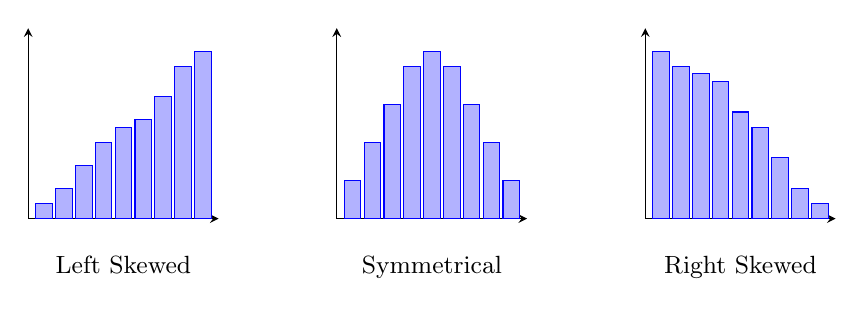
\begin{tikzpicture}

% LEFT SKEWED
\begin{axis}[
    ybar,
    bar width=6pt,
    ymin=0, ymax=25,
    xtick=\empty, ytick=\empty,
    axis lines=left,
    width=4cm, height=4cm,
    title={},
    enlarge x limits=0.1,
    name=left
]
\addplot coordinates {(1,2) (2,4) (3,7) (4,10) (5,12) (6,13) (7,16) (8,20) (9,22)};
\end{axis}
\node at (left.south) [below=10pt] {\small Left Skewed};

% SYMMETRICAL
\begin{axis}[
    at={(left.east)}, anchor=west,
    xshift=1.5cm,
    ybar,
    bar width=6pt,
    ymin=0, ymax=25,
    xtick=\empty, ytick=\empty,
    axis lines=left,
    width=4cm, height=4cm,
    title={},
    enlarge x limits=0.1,
    name=center
]
\addplot coordinates {(1,5) (2,10) (3,15) (4,20) (5,22) (6,20) (7,15) (8,10) (9,5)};
\end{axis}
\node at (center.south) [below=10pt] {\small Symmetrical};

% RIGHT SKEWED
\begin{axis}[
    at={(center.east)}, anchor=west,
    xshift=1.5cm,
    ybar,
    bar width=6pt,
    ymin=0, ymax=25,
    xtick=\empty, ytick=\empty,
    axis lines=left,
    width=4cm, height=4cm,
    title={},
    enlarge x limits=0.1,
    name=right
]
\addplot coordinates {(1,22) (2,20) (3,19) (4,18) (5,14) (6,12) (7,8) (8,4) (9,2)};
\end{axis}
\node at (right.south) [below=10pt] {\small Right Skewed};

\end{tikzpicture}
\caption*{Examples of Distribution Shapes}
\end{figure}
\par\medskip

\textbf{Practice:} A dotplot shows the number of text messages sent by 15 students in one day. Describe the distribution using SOCS.
\begin{center}
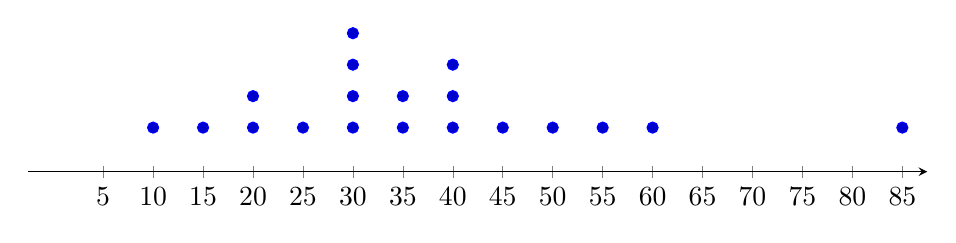
\begin{tikzpicture}
\begin{axis}[
    width=13cm,
    height=3.5cm,
    ymin=0, ymax=4,
    xmin=0, xmax=15,
    axis x line=bottom,
    axis y line=none,
    xtick={0,1,2,3,4,5,6,7,8,9,10,11,12,13,14,15,16},
    xticklabels={5,10,15,20,25,30,35,40,45,50,55,60,65,70,75,80,85},
    ytick=\empty,
    enlargelimits=0.1,
    clip=false
]
% (index, stacked count)
\addplot+[only marks, mark=*, mark size=2pt]
coordinates {
    (1,1)  % 5
    (2,1)  % 10
    (3,1) (3,2)  % 20 x2
    (4,1)  % 25
    (5,1) (5,2) (5,3) (5,4)  % 30 x3
    (6,1) (6,2)  % 35
    (7,1) (7,2) (7,3) % 40
    (8,1)  % 45
    (9,1)  % 50
    (10,1)  % 55
    (11,1) % 60
    (16,1) % 85
};
\end{axis}
\end{tikzpicture}
\end{center}
\begin{itemize}
    \item Shape: Right-skewed
    \item Outliers: 85
    \item Center: About 30
    \item Spread: Data is quite spread out, ranges from 10 to 85
\end{itemize} 
\bigskip


\section*{1.7 Summary Statistics}
We've just seen how to briefly describe a distribution of data using its shape, outliers, center, and spread. Most likely though, we're going to want to gain a bit more information about and what exactly the data is telling us. That brings us to calculating \textbf{statistics} (the name of the course itself!). \\

We can think of the population as having the true characteristics like center and spread, and the sample is what we're using to approximate these characteristics with limited data. This is really the essence of statistics: using parts of the whole to study the bigger picture. \\

So this is \textit{technically} what we mean when we refer to a statistic. Bottom line, finding statistics will let us describe distributions in much finer detail, particularly when talking about center, spread, and outliers.
\par\medskip
\begin{tcolorbox}[title=Key Formulas, colback=green!5!white, colframe=green!70!black, breakable]
\begin{itemize}
  \item \textbf{Mean}: \( \bar{x} = \frac{1}{n} \sum x_i \)
  \item \textbf{Mode}: The most commonly occurring value
  \item \textbf{Median}: Middle value
  \item \textbf{Range}: Maximum value - Minimum value
  \item \textbf{Quartiles}: Divide a data set into four equal parts
  \begin{itemize}
      \item \textbf{Q1 (First Quartile)} is the median of the lower half of the data; it marks the 25th percentile
      \item \textbf{Q3 (Third Quartile)} is the median of the upper half of the data; it marks the 75th percentile
  \end{itemize}
  \item \textbf{Interquartile Range (IQR)}: \( Q_3 - Q_1 \)
  \item \textbf{Five-Number Summary}: Minimum, Q1, Median, Q3, Maximum
  \item \textbf{Standard Deviation (SD)}: \( s = \sqrt{\frac{1}{n-1} \sum (x_i - \bar{x})^2} \)
\end{itemize}
\end{tcolorbox}
\par\medskip
\textbf{Practice:} Given the dataset = \{2, 4, 4, 6, 8\}, find the mean, median, and standard deviation. 
\begin{flushlefttab}
& Mean: \[
    \bar{x} = \frac{1}{n}\sum{x_i} = \frac{1}{5}(2+4+4+6+8) = \frac{24}{5} = 4.8
\] \\
& Median = 4 \\
& SD: \[
\begin{aligned}
s &= \sqrt{\frac{1}{n-1} \sum (x_i - \bar{x})^2} \\ &= \sqrt{\frac{1}{4} \sum (x_i - 4.8)^2} \\ &= \sqrt{\frac{1}{4}[(2-4.8)^2+(4-4.8)^2+(4-4.8)^2+(6-4.8)^2+(8-4.8)^2]} \\ &\approx 2.28
\end{aligned}
\]
\end{flushlefttab}
\par\medskip

\textbf{Practice:} Find the five-number summary for a set of measurements: 
\[
\{2,\ 3,\ 5,\ 7,\ 8,\ 9,\ 10,\ 11,\ 12,\ 13,\ 15,\ 17,\ 18,\ 20,\ 22\}
\]

\begin{flushlefttab}
& Minimum = 2 \\
& $Q_1 = 7$ \quad \text{(Median of the lower half)} \\
& $Q_2 = 11$ \quad \text{(Median of the full dataset)} \\
& $Q_3 = 17$ \quad \text{(Median of the upper half)} \\
& Maximum = 22
\end{flushlefttab}
\[
\boxed{
\text{Five-number summary: } 
\left[ \text{Min.} = 2,\ Q_1 = 7,\ \text{Median} = 11,\ Q_3 = 17,\ \text{Max.} = 22 \right]
}
\]
\bigskip

Depending on the shape of the distribution, we can say different things about its mean versus its median. In particular, see the following:

\begin{center}
\begin{minipage}{0.32\textwidth}
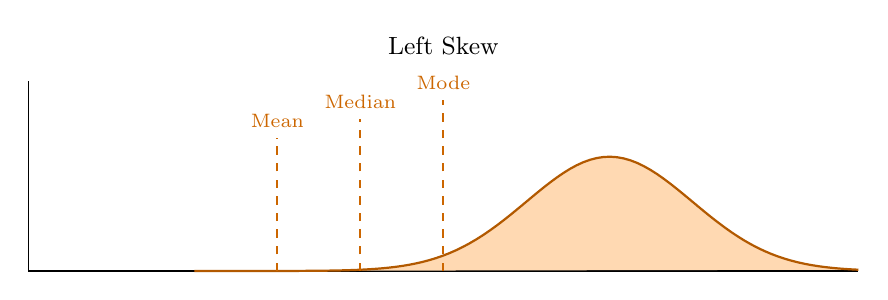
\begin{tikzpicture}
\begin{axis}[
    width=\textwidth,
    height=4cm,
    axis lines=middle,
    xtick=\empty,
    ytick=\empty,
    title={\small Left Skew},
    xmin=0, xmax=10,
    ymin=0, ymax=0.5,
    axis line style={-},
    enlargelimits=false,
    clip=false
]
\addplot[domain=2:10, samples=100, thick, orange!70!black, fill=orange!30] {0.3*exp(-(x-7)^2/2)};
\draw[dashed, thick, orange!80!black] (3,0) -- (3,0.35) node[above] {\scriptsize Mean};
\draw[dashed, thick, orange!80!black] (4,0) -- (4,0.4) node[above] {\scriptsize Median};
\draw[dashed, thick, orange!80!black] (5,0) -- (5,0.45) node[above] {\scriptsize Mode};
\end{axis}
\end{tikzpicture}
\end{minipage}
\hfill
\begin{minipage}{0.32\textwidth}
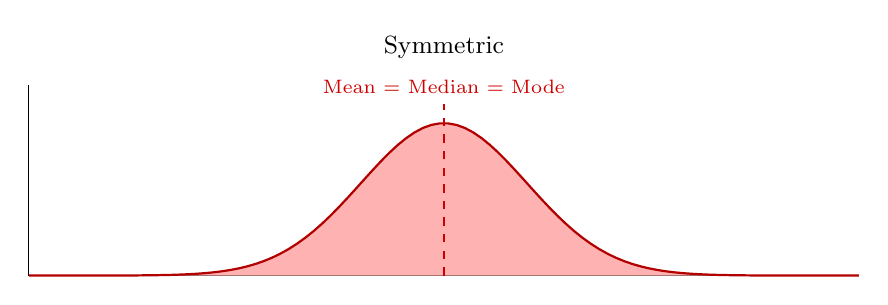
\begin{tikzpicture}
\begin{axis}[
    width=\textwidth,
    height=4cm,
    axis lines=middle,
    xtick=\empty,
    ytick=\empty,
    title={\small Symmetric},
    xmin=0, xmax=10,
    ymin=0, ymax=0.5,
    axis line style={-},
    enlargelimits=false,
    clip=false
]
\addplot[domain=0:10, samples=100, thick, red!70!black, fill=red!30] {0.4*exp(-(x-5)^2/2)};
\draw[dashed, thick, red!80!black] (5,0) -- (5,0.45) node[above] {\scriptsize Mean = Median = Mode};
\end{axis}
\end{tikzpicture}
\end{minipage}
\hfill
\begin{minipage}{0.32\textwidth}
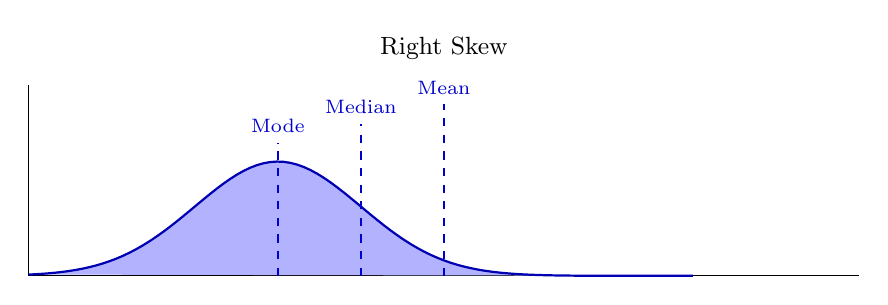
\begin{tikzpicture}
\begin{axis}[
    width=\textwidth,
    height=4cm,
    axis lines=middle,
    xtick=\empty,
    ytick=\empty,
    title={\small Right Skew},
    xmin=0, xmax=10,
    ymin=0, ymax=0.5,
    axis line style={-},
    enlargelimits=false,
    clip=false
]
\addplot[domain=0:8, samples=100, thick, blue!70!black, fill=blue!30] {0.3*exp(-(x-3)^2/2)};
\draw[dashed, thick, blue!80!black] (3,0) -- (3,0.35) node[above] {\scriptsize Mode};
\draw[dashed, thick, blue!80!black] (4,0) -- (4,0.4) node[above] {\scriptsize Median};
\draw[dashed, thick, blue!80!black] (5,0) -- (5,0.45) node[above] {\scriptsize Mean};
\end{axis}
\end{tikzpicture}
\end{minipage}
\end{center}
\bigskip

Let's talk about outliers for a bit. Specifically, the presence of outliers has a different effect on different summary statistics. 
\begin{itemize}
    \item The mean, standard deviation, and range are considered nonresistant (or non-robust) because they are influenced by outliers.
    \item The median and IQR are considered resistant (or robust), because outliers do not greatly (if at all) affect their value.
\end{itemize}
How do we detect whether a value is an outlier of the data set? There are several methods out there, but the most common is the \textbf{1.5 $\times$ IQR Criterion}. We'll demonstrate with an example.
\par\medskip

\textbf{Practice:} Determine outliers using the 1.5 $\times$ IQR Criterion.
\begin{flushlefttab}
& Dataset: \[
4,\ 5,\ 7,\ 8,\ 10,\ 11,\ 13,\ 15,\ 18,\ 19,\ 22,\ 25,\ 45
\] \\
& \textbf{Step 1: Find the Quartiles}
There are 13 values, so the median (Q\textsubscript{2}) is the 7th value:
\[
Q_2 = 13
\]
Lower half (below the median): $4,\ 5,\ 7,\ 8,\ 10,\ 11$  
Q\textsubscript{1} is the median of this group:
\[
Q_1 = \frac{7 + 8}{2} = 7.5
\]
Upper half (above the median): $15,\ 18,\ 19,\ 22,\ 25,\ 45$  
Q\textsubscript{3} is the median of this group:
\[
Q_3 = \frac{19 + 22}{2} = 20.5
\] \\
& \textbf{Step 2: Compute the IQR}
\[
\text{IQR} = Q_3 - Q_1 = 20.5 - 7.5 = 13
\] \\
& \textbf{Step 3: Apply the 1.5 $\times$ IQR Rule}
\[
\begin{aligned}
\text{Lower Bound} &= Q_1 - 1.5 \times \text{IQR} = 7.5 - 1.5 \times 13 = -12 \\
\text{Upper Bound} &= Q_3 + 1.5 \times \text{IQR} = 20.5 + 1.5 \times 13 = 40
\end{aligned}
\] \\
& \textbf{Step 4: Identify Outliers}
Any values less than the lower bound of $-12$ or greater than the upper bound of $40$ are outliers.  
Only one value exceeds 40:
\[
\boxed{45\ \text{is an outlier.}}
\]
\end{flushlefttab}
\bigskip


\section*{1.8--1.9 Comparing Distributions}
\textbf{Practice:} Compare the following boxplots of SAT math scores.
\begin{center}
\begin{tikzpicture}
\begin{axis}[
    boxplot/draw direction=y,
    ylabel={SAT Math Score},
    xtick={1,2},
    xticklabels={School A, School B},
    height=6cm,
    width=10cm,
    ymin=450, ymax=700
]
% Boxplot for School A
\addplot+[
    boxplot prepared={
        median=580,
        upper quartile=610,
        lower quartile=550,
        upper whisker=640,
        lower whisker=520
    },
] coordinates {};

% Boxplot for School B
\addplot+[
    boxplot prepared={
        median=560,
        upper quartile=630,
        lower quartile=500,
        upper whisker=680,
        lower whisker=470
    },
] coordinates {};
\end{axis}
\end{tikzpicture}
\end{center}
\bigskip
\begin{itemize}
    \item \textbf{Shape and Skewness:} School A's boxplot is more symmetric, while School B shows a slight positive skew, with a longer whisker on the upper end. This may indicate more high outlier scores at School B or a few students scoring exceptionally well.
    \item \textbf{Outliers:} Neither School A nor School B seem to have any outlier values.
    \item \textbf{Center:} School A has a higher median SAT Math score (580) compared to School B (560), suggesting that typical scores are slightly higher at School A.
    \item \textbf{Spread:} School B has a wider interquartile range (IQR = 630 - 500 = 130) than School A (IQR = 610 - 550 = 60), indicating that the middle 50\% of scores at School B are more spread out. School B also has a larger overall range (680 - 470 = 210) compared to School A (640 - 520 = 120), meaning the entire distribution of scores is more variable in School B.
    \item \textbf{Conclusion:} School A generally has higher typical scores and less variability, while School B has more spread in both the middle 50\% and overall scores. Depending on the goal (e.g., high achievers vs. consistency), each school has its strengths.
\end{itemize}


\section*{1.10 The Normal Distribution}
\begin{tcolorbox}[title=Key Formulas, colback=green!5!white, colframe=green!70!black, breakable]
\textbf{Z-score}: \( z = \frac{x - \mu}{\sigma} \), where $x$ is the observation, $\mu$ is the mean of the data, and $\sigma$ is the SD of the data.
\end{tcolorbox}
The Z-score, also sometimes called the \textbf{standardized score}, represents the number of standard deviations (SDs) away we are from the mean. 
\par\medskip

\textbf{Example:} Test score 85, scores have a mean of \( \mu = 80 \) and SD of \( \sigma = 5\). 
\par\medskip

\begin{flushlefttab}
& \boxed{z = \frac{85-80}{5} = 1 \text{(the score 85 is 1 SD above the mean)}}
\end{flushlefttab}
\par\medskip

\begin{tcolorbox}[title=Key Terms, colback=blue!5!white, colframe=blue!75!black, breakable]
The \textbf{normal distribution} is a symmetric, bell-shaped curve defined by its mean \( \mu \) and standard deviation \( \sigma \).
\end{tcolorbox}
\begin{center}
\begin{figure}
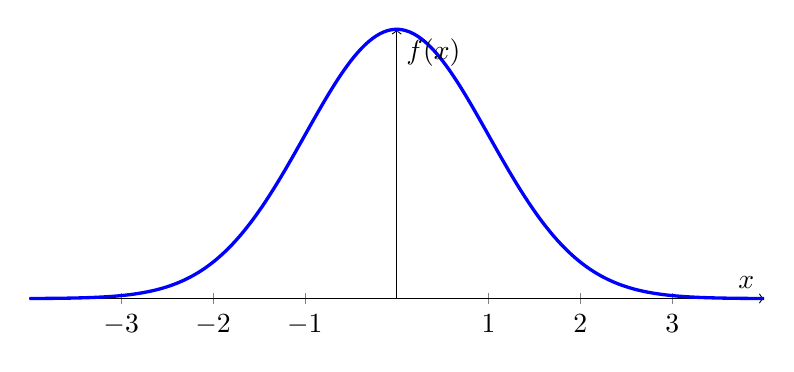
\begin{tikzpicture}
\begin{axis}[
    domain=-4:4,
    samples=200,
    axis lines=middle,
    xlabel={$x$},
    ylabel={$f(x)$},
    width=0.9\textwidth,
    height=5cm,
    xtick={-3,-2,-1,0,1,2,3},
    ytick=\empty,
    axis line style={->},
    clip=false,
    enlargelimits=false
]
\addplot [very thick, blue] {1/sqrt(2*pi)*exp(-x^2/2)};
\end{axis}
\end{tikzpicture}
\caption*{Normal Distribution}
\end{figure}
\end{center}
\par\medskip

The normal distribution is important both in the real world and in statistics. Many processes and phenomena in the natural sciences and social sciences can be found to have an approximately normal distribution. Importantly for us, we will later see that it is often used in order to make inferences about variables whose true distributions are not known. \\
\par\medskip

\begin{tcolorbox}[title=Key Results, colback=purple!5!white, colframe=purple!75!black, breakable]
\textbf{Empirical Rule:}
In a normal distribution:
\begin{itemize}
  \item 68\% of the data will be within 1 SD
  \item 95\% of the data will be within 2 SD
  \item 99.7\% of the data will be within 3 SD
\end{itemize}
\end{tcolorbox}
\par\medskip

\textbf{Practice:} Suppose the scores on a standardized exam are approximately normally distributed with a mean of 500 and a standard deviation of 100.
\begin{enumerate}
    \item What percentage of students scored between 400 and 600?
    \item What percentage of students scored between 300 and 700?
    \item What percentage of students scored above 700?
\end{enumerate}
\bigskip

\begin{enumerate}
    \item The values 400 and 600 are each one standard deviation from the mean:
    \[
    500 - 100 = 400 \quad \text{and} \quad 500 + 100 = 600
    \]
    According to the Empirical Rule, approximately 68\% of data falls within one standard deviation of the mean.
    \[
    \boxed{68\%\ \text{of students scored between 400 and 600.}}
    \]

    \item The values 300 and 700 are each two standard deviations from the mean:
    \[
    500 - 2(100) = 300 \quad \text{and} \quad 500 + 2(100) = 700
    \]
    The Empirical Rule says about 95\% of the data lies within two standard deviations.
    \[
    \boxed{95\%\ \text{of students scored between 300 and 700.}}
    \]

    \item A score above 700 is more than two standard deviations above the mean. Since 95\% of scores lie between 300 and 700, the remaining 5\% are outside this range. Because the normal distribution is symmetric, half of that 5\% is above 700:
    \[
    \frac{5\%}{2} = 2.5\%
    \]
    \[
    \boxed{2.5\%\ \text{of students scored above 700.}}
    \]
\end{enumerate}



%%%%%%%%%%%%%%%%%%%%%%%%%%%%%%%%%%%%%%%%%%%%%%%%%%%%%%%%%%%%%%%%%%%%%%



\end{document}
